\chapter{Quantizing Light: From Modes to Photons}
\label{chap:e05}

\begin{chapteropening}
In the previous chapter we quantized a single isolated harmonic oscillator: the energy can only be taken in discrete portions, the annihilation operator \(\hat a\) removes one portion, the creation operator \(\hat a^\dagger\) adds one. But that was only a ``spring.'' What a real telescope faces is an electromagnetic field that fills all of space, has color, has direction, has polarization, and fluctuates in time. What this chapter sets out to do is to replicate the success of that single harmonic oscillator of Chapter~\ref{chap:e04} onto the entire light field (tens of thousands of times over), and the method takes only one step: first decompose the light field into a set of ``modes,'' and then, to our surprise, discover that every mode is mathematically just a harmonic oscillator. At this point the word ``photon'' obtains a precise definition for the first time: it is not a little ball, but a single excitation of some mode. By the end of this chapter you will understand exactly what each ``click'' recorded by a telescope belongs to, and you will also compute one counterintuitive fact: as bright as the Sun is, each optical mode holds, on average, less than one hundredth of a photon.
\end{chapteropening}

\section{Why Decompose the Light Field into ``Modes''}
\label{sec:e05-why-modes}

Let us begin with a plain question: the electromagnetic field is a continuous thing pervading all of space, and what a telescope receives at any instant is a big blob of oscillating field. How are we to ``count it in discrete portions''?

The key to the answer is to not fixate from the outset on a continuous quantity like ``the field strength at a certain point at a certain time,'' but instead to switch to a smarter set of coordinates. Recall the Fourier analysis of Chapter~\ref{chap:e02}: any complicated stretch of sound wave can be written uniquely as a superposition of a bunch of ``pure tones'' (sinusoids of a single frequency). Pure tones are the simplest, mutually independent ``building blocks'' of the world of sound. \textbf{A mode is the electromagnetic-field version of a ``generalized pure tone.''}

A mode of the electromagnetic field is a ``building block'' labeled simultaneously by the following several things:

\begin{itemize}
  \item \textbf{Frequency}\(\ \omega\) (or color \(\nu=\omega/2\pi\)): how fast this block oscillates;
  \item \textbf{Spatial shape}\ \(u(\bm r)\): what this block looks like in space: a plane wave propagating in some direction, a diffraction-limited spot, or a guided mode in an optical fiber;
  \item \textbf{Polarization}: which way the electric-field vector points in the plane perpendicular to propagation: horizontal, vertical, or some rotation;
  \item \textbf{Time window}\ \(\Delta t\): the stretch of time this block is ``switched on.''
\end{itemize}

The reason we go to the trouble of choosing such a set of building blocks is that we want them to be \emph{mutually orthogonal, not interfering with one another}. Orthogonal here means exactly the same as ``pure tones of different frequencies are mutually independent'' in Fourier analysis: expand the field along this set of modes, and the coefficient of each mode can be measured separately, evolves separately, and is quantized separately, without any entanglement between them. Mathematically, a set of mode functions \(\{u_k(\bm r)\}\) satisfies orthonormality
\[
  \int u_i^*(\bm r)\,u_j(\bm r)\,\mathrm d^3r=\delta_{ij},
\]
where \(\delta_{ij}\) is the Kronecker delta (1 when \(i=j\), otherwise 0). With such a set of ``generalized pure tones,'' Maxwell's equations allow us to write the entire electromagnetic field as
\[
  \bm E(\bm r,t)=\sum_k\big[\,(\text{amplitude of the }k\text{th mode})\times u_k(\bm r)\,e^{-i\omega_k t}+\text{complex conjugate}\,\big].
\]
Each term oscillates independently at its own frequency \(\omega_k\); this is exactly what a ``generalized pure tone'' should look like. In the next section we fix our gaze on any one of these \(k\) and see what equation of motion its amplitude obeys.

\section{The Key Step: Every Mode Is a Harmonic Oscillator}
\label{sec:e05-mode-is-oscillator}

Now lock attention onto a single mode \(k\). Its spatial shape \(u_k(\bm r)\) is fixed; the only thing still in motion is its amplitude, call it \(q_k(t)\). What we will do is substitute this single-mode field into the energy density of the electromagnetic field, integrate over space, and see what the total energy it carries looks like. This step, in standard electrodynamics, is called the ``mode expansion of the field energy''; many textbooks (such as the section on cavity modes in Jackson's \emph{Classical Electrodynamics}, or the first chapter of any introductory quantum-optics book) do it. But it is precisely the \emph{foundation} of this chapter, and skipping over it would leave the self-taught reader unable to prove it for themselves, so we walk through this piece of algebra exactly as it is. Only three facts are really needed, and we call each of them by name as we go.

\textbf{Fact one: the electromagnetic energy-density formula.} The total energy of a free electromagnetic field enclosed in a volume is (in CGS units)
\[
  U=\frac{1}{8\pi}\int\big(\bm E^2+\bm B^2\big)\,\mathrm d^3r,
\]
the electric-field term and the magnetic-field term contributing symmetrically half each; this is a result you learned back in general-physics electromagnetism, in units of erg.

\textbf{Fact two: how to write the single-mode field.} Keep only the \(k\)th mode in the expression. Taking it to be a real standing wave (a cavity mode), the electric field can be written as ``spatial shape \(\times\) time-varying amplitude'':
\[
  \bm E_k(\bm r,t)=-\,c_1\,\dot q_k(t)\,\bm u_k(\bm r),
\]
where \(\bm u_k\) is the orthonormal mode function of the previous section, \(q_k(t)\) is the amplitude coordinate we are tracking, and \(c_1\) is a proportionality factor containing only constants (\(4\pi\), \(c\), etc.); we carry it along for now, and it will in the end be absorbed into the definition of \(q_k\).

\textbf{Fact three: Maxwell's equations tie \(\dot{\bm E}\) and \(\bm B\) together.} In vacuum \(\nabla\times\bm B=\tfrac1c\,\partial_t\bm E\), so the magnetic field is determined by the time derivative of the electric field. Substituting \(\bm E_k\propto\dot q_k\,\bm u_k\) of fact two, the right side \(\propto\ddot q_k\,\bm u_k\); for a mode oscillating harmonically at \(\omega_k\), \(\ddot q_k=-\omega_k^2 q_k\), so the time part of the magnetic field is proportional to \(q_k(t)\) itself, while the spatial part is determined by \(\nabla\times\bm u_k\):
\[
  \bm B_k(\bm r,t)=c_2\,q_k(t)\,\big[\nabla\times\bm u_k(\bm r)\big].
\]
Here the mode also satisfies the Helmholtz equation \(\nabla^2\bm u_k=-(\omega_k^2/c^2)\,\bm u_k\) (``the degree of curvature of the spatial shape sets the frequency''), which will presently help us compute the spatial integral of the magnetic-field term into a number containing \(\omega_k^2\).

Now substitute facts two and three into the integral of fact one. The electric-field term gives
\[
  \frac1{8\pi}\int\bm E_k^2\,\mathrm d^3r
  =\frac{c_1^2}{8\pi}\,\dot q_k^{\,2}\int|\bm u_k|^2\,\mathrm d^3r
  =\frac{c_1^2}{8\pi}\,\dot q_k^{\,2},
\]
where the last step used precisely the \emph{orthonormality} \(\int|\bm u_k|^2\,\mathrm d^3r=1\) of the previous section, at once turning the spatial integral into 1. Likewise, doing the same integral in the magnetic-field term (using \(\int|\nabla\times\bm u_k|^2\,\mathrm d^3r=(\omega_k^2/c^2)\int|\bm u_k|^2\,\mathrm d^3r=\omega_k^2/c^2\), a step that uses the Helmholtz equation) gives
\[
  \frac1{8\pi}\int\bm B_k^2\,\mathrm d^3r
  =\frac{c_2^2}{8\pi}\,q_k^{\,2}\cdot\frac{\omega_k^2}{c^2}
  \ \propto\ \omega_k^2\,q_k^{\,2}.
\]
So the electric-field term \(\propto\dot q_k^{\,2}\) and the magnetic-field term \(\propto\omega_k^2 q_k^{\,2}\); putting the two together, the energy takes on the ``kinetic plus potential'' form of a harmonic oscillator:
\[
  U_k=(\text{constant}_1)\,\dot q_k^{\,2}+(\text{constant}_2)\,\omega_k^2\,q_k^{\,2}.
\]
The last step is the crucial one: those two constants (both assembled from \(c_1,c_2,4\pi,c\), etc.) are \emph{not} irrelevant. We \textbf{redefine \(q_k\)} so that it absorbs these constants together (physically this can always be done: it is just multiplying the amplitude by a constant factor). Choosing this normalization is defining \(q_k\) to be the \emph{canonical coordinate} of this mode, with the effective mass taken to be 1. Then both coefficients become exactly \(\tfrac12\), and the energy equals exactly
\[
  H_k=\tfrac12\,\dot q_k^{\,2}+\tfrac12\,\omega_k^2\,q_k^{\,2}.
\]
Read this line three times. It is \emph{identical} to the energy of that mass-1 spring of Chapter~\ref{chap:e04}, \(H=\tfrac12\dot q^2+\tfrac12\omega^2 q^2\); note that this is an exact \emph{equality}, not ``proportional to'': that once-ambiguous proportionality constant has already been swallowed by our definition of \(q_k\), so the effective mass is exactly 1 and not some other coefficient. In other words:

\begin{quote}
\textbf{Every electromagnetic field mode is, mathematically, a harmonic oscillator of frequency \(\omega_k\).}
\end{quote}

This is the pivot of the whole chapter. Once we grant this sentence, we \emph{need invent nothing new}; we simply apply, word for word, the quantization we did for the harmonic oscillator in Chapter~\ref{chap:e04} to each mode. In Chapter~\ref{chap:e04} we packaged \(q,\dot q\) into an annihilation operator \(\hat a\) and a creation operator \(\hat a^\dagger\). Here we do the same for the \(k\)th mode, obtaining a pair \(\hat a_k,\hat a_k^\dagger\). Because different modes are mutually orthogonal and do not interfere, their operator commutation relations are

\begin{equation}
  [\hat a_i,\hat a_j^\dagger]=\delta_{ij},\qquad
  [\hat a_i,\hat a_j]=0,\qquad
  \hat n_k=\hat a_k^\dagger\hat a_k .
  \label{eq:e05-commutator}
\end{equation}
\begin{formulaexplain}
\(\hat a_k^\dagger,\hat a_k\) add and remove one photon in the \(k\)th mode; \(\delta_{ij}\) says that only the creation and annihilation of the \emph{same} mode leave a quantum correction behind, and different modes are completely independent; \(\hat n_k\) counts how many photons are in the \(k\)th mode.
\end{formulaexplain}

Let us account for each symbol. \(\hat a_k\) is the annihilation operator of the \(k\)th mode, dimensionless; it lowers the excitation number of that mode by one. \(\hat a_k^\dagger\) is the creation operator, which raises the excitation number by one. The physical meaning of the commutator \(\delta_{ij}\) is one of the key points of this chapter: when \(i\neq j\), \([\hat a_i,\hat a_j^\dagger]=0\), meaning ``photons in the red-light mode'' and ``photons in the blue-light mode'' are two utterly unrelated ledgers that can be counted separately; this is exactly the reward for our having chosen \emph{orthogonal} modes in the first place. The eigenvalues of the number operator \(\hat n_k=\hat a_k^\dagger\hat a_k\) are \(N_k=0,1,2,\dots\), pure integers with no units, and it counts ``how many portions of excitation are in the \(k\)th mode right now.''

One portion of excitation is one photon. At this point, ``photon'' finally has an unambiguous definition: a photon is not a bullet flying through space, but \emph{the energy of one definite mode (a definite frequency, a definite spatial shape, a definite polarization) raised by one whole portion}. The same photon necessarily belongs to some mode; asking ``where is this photon'' is equivalent to asking ``which mode does it belong to.''

\section{The Positive-Frequency Field Operator: Photons Make Their Formal Entrance}
\label{sec:e05-field-operator}

Reassembling the annihilation operators of each mode from the previous section according to spatial shape and frequency yields the quantized electric field. What a detector truly uses when it ``absorbs a photon'' is the half of the electric field containing only \(\hat a_k\) (annihilation), called the \textbf{positive-frequency field operator}:

\begin{equation}
  \hat E^{(+)}(\bm r,t)=\sum_k \mathcal E_k\,u_k(\bm r)\,e^{-i\omega_k t}\,\hat a_k .
  \label{eq:e05-field-expansion}
\end{equation}
\begin{formulaexplain}
The light field written as a sum over a bunch of modes: in the \(k\)th term, \(\mathcal E_k\) is the normalization coefficient for ``how strong one photon is,'' \(u_k(\bm r)\) is the spatial shape of the mode, \(e^{-i\omega_k t}\) is its oscillation, and \(\hat a_k\) \emph{removes one photon} from this mode. The whole expression is ``the light the detector sees.''
\end{formulaexplain}

Let us make each symbol clear; this equation is the foundation of all the later chapters.

\begin{itemize}
  \item \(\hat E^{(+)}(\bm r,t)\): the positive-frequency electric-field operator, containing the ``annihilation'' part. \(\bm r\) is position (units cm), \(t\) is time (units s).
  \item \(\mathcal E_k\): the single-photon field strength, that is, the normalization factor for ``how big an electric field one photon in this mode corresponds to.'' It converts the dimensionless operator \(\hat a_k\) into a genuine field strength (in CGS, units \(\mathrm{statvolt\,cm^{-1}}\)). It is set by the mode's frequency and effective volume; by order of magnitude \(\mathcal E_k\propto\sqrt{\hbar\omega_k/V}\); here \(V\) is the effective volume of the mode (units cm\(^3\)), \(\hbar=h/2\pi\) is the reduced Planck constant (\(h\) the Planck constant, see Section~\ref{sec:e05-occupation}), and the numerator \(\hbar\omega_k=h\nu_k\) is exactly the energy of one photon. The higher the frequency and the smaller the mode volume, the stronger the field of a single photon.
  \item \(u_k(\bm r)\): the spatial mode function of the \(k\)th mode, dimensionless (already orthonormalized per the previous section), carrying ``what this block looks like and which way it goes.''
  \item \(e^{-i\omega_k t}\): the time oscillation of this mode, \(\omega_k=2\pi\nu_k\) being the angular frequency (units \(\mathrm{rad\,s^{-1}}\)). The sign convention makes it the ``positive-frequency'' part.
  \item \(\hat a_k\): the annihilation operator. It is the only ``quantum'' ingredient in this equation; because of it, the electric field is no longer a number but an operator that can change the photon number.
\end{itemize}

Where did the other half (the part containing only the creation operator \(\hat a_k^\dagger\)) go? It is the Hermitian conjugate of \eqref{eq:e05-field-expansion}:
\[
  \hat E^{(-)}(\bm r,t)=\big[\hat E^{(+)}(\bm r,t)\big]^\dagger
  =\sum_k \mathcal E_k^*\,u_k^*(\bm r)\,e^{+i\omega_k t}\,\hat a_k^\dagger .
\]
Adding the two halves, \(\hat{\bm E}=\hat E^{(+)}+\hat E^{(-)}\), is the complete, observable (Hermitian) electric-field operator. Why split them apart? Because \textbf{photodetection is essentially absorption}: an electron in the detector is ``knocked'' out by light by \emph{taking away} one photon from the light field, and this process uses only the annihilation operator \(\hat a_k\), that is, only \(\hat E^{(+)}\). And so we obtain a sentence that runs through the whole book:

\begin{quote}
\textbf{Detecting one photon is decreasing the photon number in some mode by one}; mathematically it is \(\hat E^{(+)}\) (containing \(\hat a_k\)) acting on the light state.
\end{quote}

A telescope never reads out \(\hat a_k\) or \(\hat E\) directly; what it reads out are time stamps, pixels, energy channels, polarization channels, all of which are products of \(\hat n_k\), or of correlations of several \(\hat n\), after passing through the instrument response. But conceptually, behind every click stands an \(\hat a_k\): some mode, one photon fewer.

\section{Number States of Light: Fock States}
\label{sec:e05-fock}

Since every mode is a harmonic oscillator, the energy eigenstates of the harmonic oscillator naturally upgrade into the energy eigenstates of the light field. The state in which the \(k\)th mode has exactly \(N_k\) photons is written \(|N_k\rangle\), satisfying \(\hat n_k|N_k\rangle=N_k|N_k\rangle\). Specifying the occupation numbers of all modes together yields a \textbf{number state} of the entire light field, also called a \textbf{Fock state}:

\begin{equation}
  |\{N_k\}\rangle=|N_1,N_2,N_3,\dots\rangle,
  \qquad
  \hat n_k\,|\{N_k\}\rangle=N_k\,|\{N_k\}\rangle .
  \label{eq:e05-fock}
\end{equation}
\begin{formulaexplain}
A Fock state is a ``roll call'': \(N_1\) photons in mode 1, \(N_2\) photons in mode 2, \ldots; every number is definite, with no fluctuation. It is the exact answer-state to the question ``exactly how many photons are in each mode.''
\end{formulaexplain}

Here \(N_k=0,1,2,\dots\) is the photon number of the \(k\)th mode, a pure integer with no units. The physical meaning of a number state is very clean: it \emph{pins down the photon number of every mode}, with no fluctuation whatsoever. For example, \(|0,0,\dots\rangle\) (all modes empty) is the electromagnetic vacuum; \(|0,1,0,\dots\rangle\) is the single-photon state of ``only one photon in mode 2, all others empty.'' Any Fock state can be built up with creation operators, just as in Chapter~\ref{chap:e04} we climbed the energy ladder rung by rung with \(\hat a^\dagger\):
\[
  |\{N_k\}\rangle=\prod_k\frac{(\hat a_k^\dagger)^{N_k}}{\sqrt{N_k!}}\,|0\rangle,
\]
where \(\sqrt{N_k!}\) is the normalization factor (its origin identical to the single-mode case of Chapter~\ref{chap:e04}, normalized once for each mode here). Fock states are the ``coordinate basis'' for understanding all states of light: the coherent states and thermal states to come will both be written as superpositions or mixtures of Fock states. And the most important lesson they teach is: the information carried by light hides in the \emph{photon number} and the \emph{correlations of photon number}, not in a continuous waveform.

\section{Exactly How Many Modes Are in One Channel}
\label{sec:e05-mode-count}

Here is the pitfall most easily stepped into in astronomical observation: in a data file, ``one channel'' (one pixel, one time bin, one filter) is almost \emph{never} a single quantum mode, but a sum of very many modes. To get the physics right, we must first learn to count: how many independent modes are packed into one observing channel?

The idea is ``multiply the resolvable cells in phase space.'' The three kinds of mode labels (time, space, polarization) are mutually independent, so the total mode count is the product of each one's cell count. Let us count term by term.

\paragraph{Time modes.} A wave packet of bandwidth \(\Delta\nu\) has a time over which it ``remembers its own phase'' (the coherence time) of about \(\tau_c\simeq1/\Delta\nu\) (this is exactly the Fourier conclusion of Chapter~\ref{chap:e02}, ``shorter in time, wider in spectrum''). So an observing time window of length \(\Delta t\) holds about
\[
  \frac{\Delta t}{\tau_c}
\]
mutually independent time modes; every \(\tau_c\), the field ``forgets'' its previous phase, equivalent to switching to a fresh building block.

\paragraph{Spatial modes.} Diffraction determines how large an ``\'etendue'' (area \(\times\) solid angle) one spatial mode occupies. A beam of diffraction-limited single-mode light has an area-solid-angle product of about \(A\Omega\sim\lambda^2\) (another way of writing the diffraction limit \(\Delta\theta\sim\lambda/D\)). If the telescope together with the back end receives an \'etendue \(A\Omega\), then the number of spatial modes it holds is about
\[
  \frac{A\Omega}{\lambda^2}.
\]
A diffraction-limited imaging of a point source gives \(A\Omega\sim\lambda^2\), that is, a single spatial mode; whereas an image smeared out by atmospheric jitter (seeing), or coupled into a thick fiber, or falling on a large pixel, takes in many spatial modes at once.

\paragraph{Polarization modes.} The electric field has two independent polarization directions perpendicular to propagation. If the observation does not project the polarization onto a single channel, then multiply again by the polarization mode count \(N_{\rm pol}\) (usually 1 or 2).

Multiplying the three terms gives the effective mode count:

\begin{equation}
  M\simeq
  \underbrace{\frac{\Delta t}{\tau_c}}_{\text{time}}\,
  \underbrace{\frac{A\Omega}{\lambda^2}}_{\text{space}}\,
  \underbrace{N_{\rm pol}}_{\text{polarization}},
  \qquad
  \tau_c\simeq\frac1{\Delta\nu}\simeq\frac{\lambda^2}{c\,\Delta\lambda}.
  \label{eq:e05-mode-number}
\end{equation}
\begin{formulaexplain}
Effective mode count = number of time cells \(\times\) number of spatial cells \(\times\) number of polarizations. It tells you that an observing channel is really the average of \(M\) quantum modes; the larger \(M\) is, the more fiercely the quantum fluctuations are diluted.
\end{formulaexplain}

Where does that last \(\tau_c\simeq\lambda^2/(c\,\Delta\lambda)\) come from? Differentiating \(\nu=c/\lambda\), \(|\mathrm d\nu|=(c/\lambda^2)\,|\mathrm d\lambda|\), that is, the bandwidth conversion \(\Delta\nu\simeq c\,\Delta\lambda/\lambda^2\) (consistent with the notation of Chapter~\ref{chap:e02}); taking the reciprocal gives \(\tau_c\simeq\lambda^2/(c\,\Delta\lambda)\).

Let us plug in real numbers to get a feel. Take visible light \(\lambda=500\,\mathrm{nm}=5\times10^{-5}\,\mathrm{cm}\), filter bandwidth \(\Delta\lambda=1\,\mathrm{nm}=10^{-7}\,\mathrm{cm}\), and \(c=3\times10^{10}\,\mathrm{cm\,s^{-1}}\):
\[
  \Delta\nu\simeq\frac{c\,\Delta\lambda}{\lambda^2}
  =\frac{(3\times10^{10})(10^{-7})}{(5\times10^{-5})^2}\,\mathrm{Hz}
  \simeq1.2\times10^{12}\,\mathrm{Hz},
  \qquad
  \tau_c\simeq\frac1{\Delta\nu}\simeq0.8\,\mathrm{ps}.
\]
The coherence time is less than 1 picosecond! Yet even the fastest photodetectors have a time response on the order of \(100\,\mathrm{ps}\sim1\,\mathrm{ns}\). This means that even with a detector that ``runs blazingly fast,'' one time bin has already packed in \(\Delta t/\tau_c\sim10^2\)--\(10^3\) independent time modes. Adding on the spatial modes smeared by seeing, an astronomical channel readily becomes a sum of \emph{thousands upon thousands of modes}. Remember this sentence; it will later explain why the bunching and non-classical signals of astronomical light are always ``diluted'' so shallowly:

\begin{quote}
\textbf{``One channel'' in astronomy is usually not a single quantum mode, but a sum of many modes.}
\end{quote}

\section{Single-Mode Boson Occupation: Every Mode Is Actually Quite Dim}
\label{sec:e05-occupation}

One last order of magnitude will thoroughly change your intuition about ``how bright a star is.'' The question is: for the continuum light of a star, on average \emph{how many photons are in each mode}?

Treat a mode of some frequency \(\nu\) as a harmonic oscillator in equilibrium with a heat bath at brightness temperature \(T_b\). When this mode has \(N\) photons the energy is \(N h\nu\) (the energy ladder of Chapter~\ref{chap:e04}, taking the part above the zero-point energy here). In thermal equilibrium the probability of \(N\) photons appearing is given by the Boltzmann weight, proportional to \(e^{-Nh\nu/k_{\rm B}T_b}\). For notational convenience, write
\[
  x\equiv e^{-h\nu/k_{\rm B}T_b}\quad(0<x<1),\qquad
  P(N)=\frac{x^N}{\sum_{M=0}^{\infty}x^M}.
\]
The denominator is a geometric series, and using the summation formula for common ratio \(x\), \(\sum_{M=0}^{\infty}x^M=1/(1-x)\) (convergent since \(0<x<1\)), the normalized probability is the geometric distribution
\[
  P(N)=(1-x)\,x^N .
\]
Now compute the mean occupation \(\bar n_\nu=\langle N\rangle=\sum_{N=0}^{\infty}N\,P(N)\). The key is that step involving the sum with \(N\). Use a standard trick: differentiate the geometric series term by term,
\[
  \sum_{N=0}^{\infty}N\,x^N
  =x\,\frac{\mathrm d}{\mathrm dx}\sum_{N=0}^{\infty}x^N
  =x\,\frac{\mathrm d}{\mathrm dx}\!\left(\frac1{1-x}\right)
  =\frac{x}{(1-x)^2}.
\]
Substituting back, that \((1-x)\) cancels exactly once:
\[
  \bar n_\nu=(1-x)\sum_{N=0}^{\infty}N\,x^N
  =(1-x)\cdot\frac{x}{(1-x)^2}
  =\frac{x}{1-x}
  =\frac1{\,1/x-1\,}.
\]
Substituting \(1/x=e^{+h\nu/k_{\rm B}T_b}\) back in gives the closing formula of this chapter, the single-mode boson occupation, the familiar factor in the Planck distribution:

\begin{equation}
  \bar n_\nu=\frac1{\exp(h\nu/k_{\rm B}T_b)-1}.
  \label{eq:e05-occupation}
\end{equation}
\begin{formulaexplain}
\(\bar n_\nu\) is ``how many photons are in each mode on average.'' \(h\nu\) is the energy of one photon, \(k_{\rm B}T_b\) is the thermal energy corresponding to the brightness temperature; the larger the ratio of the two, the exponentially smaller the occupation. It measures ``how many photons per mode,'' not ``how many photons in total.''
\end{formulaexplain}

Let us account for each unit. Both \(h\nu\) and \(k_{\rm B}T_b\) are energies (units erg in CGS): \(h\) is the Planck constant, \(k_{\rm B}\) the Boltzmann constant, and \(T_b\) the brightness temperature (units K). \(\bar n_\nu\) is dimensionless, simply a pure ``mean photon number.''

Substitute the Sun. Take a stellar surface brightness temperature \(T_b=5800\,\mathrm{K}\) and wavelength \(\lambda=500\,\mathrm{nm}\). The photon energy is \(h\nu=hc/\lambda\). Using the convenient value \(hc\simeq1240\,\mathrm{eV\,nm}\), we get \(h\nu\simeq1240/500\simeq2.48\,\mathrm{eV}\); the thermal energy \(k_{\rm B}T_b\simeq(8.62\times10^{-5}\,\mathrm{eV\,K^{-1}})(5800\,\mathrm{K})\simeq0.50\,\mathrm{eV}\). So the ratio that decides everything is
\[
  \frac{h\nu}{k_{\rm B}T_b}\simeq\frac{2.48}{0.50}\simeq5.0 .
\]
Substituting into \eqref{eq:e05-occupation}:
\[
  \bar n_\nu\simeq\frac1{e^{5}-1}=\frac1{148.4-1}\simeq6.8\times10^{-3}
  \approx7\times10^{-3}.
\]
Each optical mode holds, on average, only about \emph{seven thousandths of a photon}. In other words, the vast majority of modes are \emph{empty} during the vast majority of coherence-time windows, with only occasionally a photon popping up in some mode. This is the ``few-photon-per-mode regime'' in which visible-light astronomy sits.

Here we must sharply distinguish two things, or we will be led astray by the intuition that ``the Sun is so bright'':

\begin{quote}
\textbf{A high total photon rate does not at all mean many photons per mode.}
\end{quote}

The Sun pours a vast number of photons into the telescope each second because it simultaneously lights up an \emph{astronomically large} number of modes (\(M\) is enormous, see the previous section), not because each mode is very ``full.'' Each mode itself is actually quite dim, \(\bar n_\nu\sim10^{-2}\). This order of magnitude changes with wavelength: in the near-infrared at \(\lambda=1\,\mu\mathrm{m}\), \(h\nu/k_{\rm B}T_b\) halves and \(\bar n_\nu\) rises to about \(0.09\); in the mid-infrared at \(10\,\mu\mathrm{m}\) it can exceed 1; while in the radio and millimeter bands, because \(h\nu\ll k_{\rm B}T_b\), one enters the strong-occupation, near-classical wave regime of \(\bar n_\nu\gg1\) (the Rayleigh--Jeans regime). Astrophysical masers (such as water masers and hydroxyl masers) are even more extreme examples: their brightness temperatures in the radio/millimeter bands can reach above \(10^{12}\)\,K, so the single-mode occupation \(\bar n_\nu\) is enormous, photons crowd into the same mode, and the behavior is almost purely a classical wave. Figure~\ref{fig:e05-mode-occupation} draws this curve varying with wavelength and brightness temperature (only three ordinary blackbody curves are drawn; the maser brightness temperature is far off the chart).

\begin{figure}[tbp]
\centering
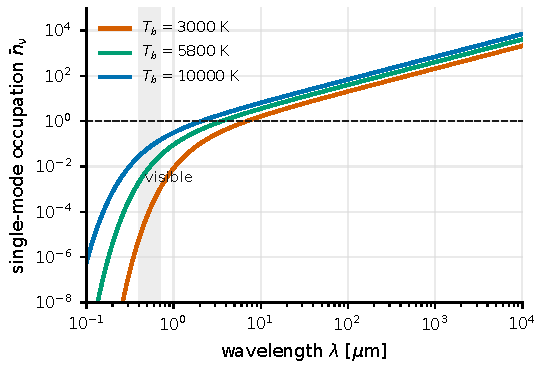
\includegraphics[width=0.82\linewidth]{figures/generated/chapter_03/ch03_blackbody_mode_occupation.pdf}
\caption{The single-mode occupation \(\bar n_\nu\) of three blackbodies of different brightness temperature (3000, 5800, 10000\,K) as a function of wavelength; the gray band marks the visible band, the dashed line marks \(\bar n_\nu=1\). Within the visible gray band, even at a brightness temperature of solar order, \(\bar n_\nu\) is far below 1 (\(\sim10^{-2}\)), showing that optical stellar light sits in the few-photon-per-mode regime; toward the long-wavelength (infrared, millimeter) end, the curves of each temperature cross the \(\bar n_\nu=1\) dashed line in turn, entering the strong-occupation, near-classical (Rayleigh--Jeans) limit of \(h\nu\ll k_{\rm B}T_b\).}
\label{fig:e05-mode-occupation}
\end{figure}

Why does this ``every mode is quite dim'' matter so much? Because it is precisely the starting point of the next several chapters. Since a coherence-time window usually contains no photon, and only occasionally one, what carries the spatial information of the celestial object is often the mode occupied by that single detected photon; this directly leads to the statistics of weak thermal light, the correlation of photons arriving in pairs, and the idea of quantum super-resolution beyond the diffraction limit. Carrying the sentence ``every mode of the Sun is actually quite dim,'' we can enter the next stage: seeing what statistical fingerprints these sparse photons leave on the detector.

\section{Chapter Summary}
\label{sec:e05-summary}

\begin{itemize}
  \item \textbf{Modes are the ``generalized pure tones'' of the light field.} Expanding the electromagnetic field along a set of orthogonal modes (frequency, spatial shape, polarization, time window) is a generalization of the Fourier idea to the electromagnetic field, with the benefit that each mode is independent and can be quantized separately.
  \item \textbf{Every mode is a harmonic oscillator.} This is the pivot of the whole chapter: the quantization of Chapter~\ref{chap:e04} is applied unchanged, giving the per-mode \(\hat a_k,\hat a_k^\dagger\), the commutation relation \([\hat a_i,\hat a_j^\dagger]=\delta_{ij}\), and the number operator \(\hat n_k=\hat a_k^\dagger\hat a_k\).
  \item \textbf{Photon = one excitation of some mode.} The only quantum ingredient in the positive-frequency field operator \(\hat E^{(+)}=\sum_k\mathcal E_k u_k(\bm r)e^{-i\omega_k t}\hat a_k\) is \(\hat a_k\); detecting one photon is decreasing the photon number in some mode by one. \(\hat E^{(-)}\) is its Hermitian conjugate.
  \item \textbf{The Fock state \(|\{N_k\}\rangle\)} pins down the photon number of every mode and is the coordinate basis for understanding all states of light.
  \item \textbf{An observing channel is often a sum of many modes}: \(M\simeq(\Delta t/\tau_c)(A\Omega/\lambda^2)N_{\rm pol}\), readily reaching thousands upon thousands in the visible.
  \item \textbf{Optical stellar light sits in the few-photon-per-mode regime}: \(\bar n_\nu=[\exp(h\nu/k_{\rm B}T_b)-1]^{-1}\), and at solar order \(\bar n_\nu\approx7\times10^{-3}\). A high total photon rate \(\neq\) many photons per mode.
\end{itemize}

\medskip
\noindent\textbf{Questions to Ponder.}
\begin{enumerate}
  \item If you widened the filter bandwidth \(\Delta\lambda\) by a factor of 10, how would the coherence time \(\tau_c\) and the number of time modes in a \(\Delta t\) time window each change?
  \item A thick fiber receiving a seeing-smeared image, versus a diffraction-limited imager, which has the larger spatial mode count \(A\Omega/\lambda^2\)? What does this mean for ``how deep the quantum fluctuations we see are''?
  \item For the same star, why does the ``few-photon-per-mode'' picture fail when observing at \(10\,\mu\mathrm{m}\) in the mid-infrared? Use \eqref{eq:e05-occupation} to estimate \(\bar n_\nu\) in this case.
\end{enumerate}
